%!TEX program = xelatex
\documentclass[cn,normal,11pt]{../elegantnote}

\usepackage{tikz}

\title{TikZ \& PGF 学习笔记}

\author{\href{https://github.com/lightjameslyy/}{刘涛}}
\institute{中科院计算所}
\version{0.1}
\date{\today}


\begin{document}
\maketitle

\setlist[itemize]{label=$\circ$}

\begin{enumerate}
    \item straight path。有两种格式:

    \tikz \draw[thick, rounded corners=8pt]
        (0,0) -- (0,2) -- (1,3.25) -- (2,2) -- (2,0) -- (0,2) -- (2,2) -- (0,0) -- (2,0);
    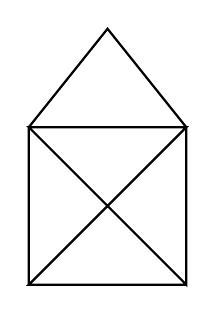
\begin{tikzpicture}
        \draw[thick]
        (0,0) -- (0,2) -- (1,3.25) -- (2,2) -- (2,0) -- (0,2) -- (2,2) -- (0,0) -- (2,0);
    \end{tikzpicture}

    \item curved path:有 1 到 2 个 control 点。比如曲线的起止点是 x 和 y,control 点是 z 和 w。那么在 x 点,曲线的斜率正好是 x 到 z,在 y 点是 w 到 y。

    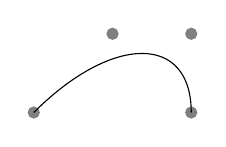
\begin{tikzpicture}
        \filldraw [gray] 
            (0,0) circle [radius=2pt]
            (1,1) circle [radius=2pt]
            (2,1) circle [radius=2pt]
            (2,0) circle [radius=2pt];
        \draw (0,0) .. controls (1,1) and (2,1) .. (2,0);
    \end{tikzpicture}

    \item 用 controls 画一个半圆:
    
    \begin{tikzpicture}
        \filldraw [gray] 
            (-1,0.555) circle [radius=1pt]
            (-0.555,1) circle [radius=1pt]
            (0.555,1) circle [radius=1pt]
            (1,0.555) circle [radius=1pt];
        \draw (-1.5,0) -- (1.5,0);
        \draw (0,-1.5) -- (0,1.5);
        \draw (-1,0) .. controls (-1,0.555) and (-0.555,1) .. (0,1)
            .. controls (0.555,1) and (1,0.555) .. (1,0);
    \end{tikzpicture}

    \item 上面画圆的方法有点复杂,可以直接用 circle 或 ellipse 路径:
    
    \tikz \draw (0,0) circle [radius=10pt];
    \tikz \draw (0,0) ellipse [x radius=20pt, y radius=10pt];

    \item 一个更直观的画圆的方法:
    
    \begin{tikzpicture}
        \draw (-1.5,0) -- (1.5,0);
        \draw (0,-1.5) -- (0,1.5);
        \draw (0,0) circle [radius=1cm];
    \end{tikzpicture}

    \item rectangle:

    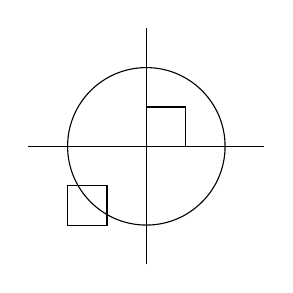
\begin{tikzpicture}
        \draw (-1.5,0) -- (1.5,0);
        \draw (0,-1.5) -- (0,1.5);
        \draw (0,0) circle [radius=1cm];
        \draw (0,0) rectangle (0.5,0.5);
        \draw (-1,-1) rectangle (-0.5,-0.5);
    \end{tikzpicture}

    \item grid:

    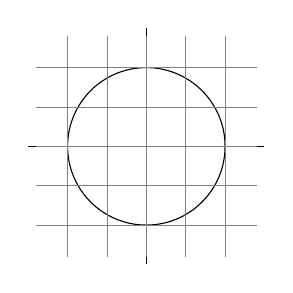
\begin{tikzpicture}
        \draw (-1.5,0) -- (1.5,0);
        \draw (0,-1.5) -- (0,1.5);
        \draw (0,0) circle [radius=1cm];
        \draw[step=.5cm,gray,very thin] (-1.4,-1.4) grid (1.4,1.4);
    \end{tikzpicture}

    \item arc path:
    
    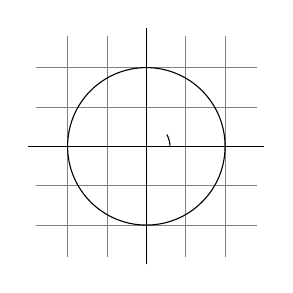
\begin{tikzpicture}
        \draw[step=.5cm,gray,very thin] (-1.4,-1.4) grid (1.4,1.4);
        \draw (-1.5,0) -- (1.5,0);
        \draw (0,-1.5) -- (0,1.5);
        \draw (0,0) circle [radius=1cm];
        \draw (3mm,0mm) arc [start angle=0, end angle=30, radius=3mm];
    \end{tikzpicture}
    \tikz \draw (0,0)
        arc [start angle=0, end angle=315,
        x radius=1.75cm, y radius=1cm];

    \item 通过设置 scale 实现缩放:
    
    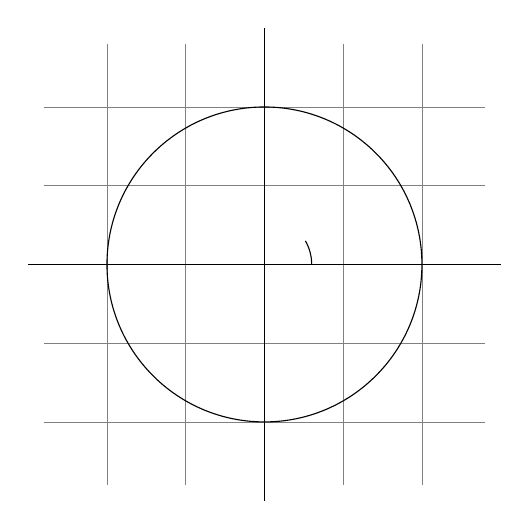
\begin{tikzpicture}[scale=2]
        \draw[step=.5cm,gray,very thin] (-1.4,-1.4) grid (1.4,1.4);
        \draw (-1.5,0) -- (1.5,0);
        \draw (0,-1.5) -- (0,1.5);
        \draw (0,0) circle [radius=1cm];
        \draw (3mm,0mm) arc [start angle=0, end angle=30, radius=3mm];
    \end{tikzpicture}

    \item 使用 clip 截取图的一部分:视窗可以是矩形、圆形……
    
    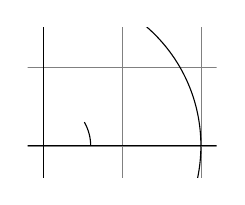
\begin{tikzpicture}[scale=2]
        \clip (-0.1,-0.2) rectangle (1.1,0.75);
        \draw[step=.5cm,gray,very thin] (-1.4,-1.4) grid (1.4,1.4);
        \draw (-1.5,0) -- (1.5,0);
        \draw (0,-1.5) -- (0,1.5);
        \draw (0,0) circle [radius=1cm];
        \draw (3mm,0mm) arc [start angle=0, end angle=30, radius=3mm];
    \end{tikzpicture}
    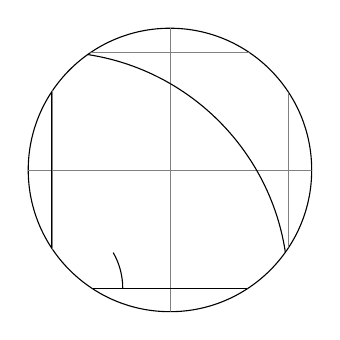
\begin{tikzpicture}[scale=3]
        \clip[draw] (0.5,0.5) circle (.6cm);
        \draw[step=.5cm,gray,very thin] (-1.4,-1.4) grid (1.4,1.4);
        \draw (-1.5,0) -- (1.5,0);
        \draw (0,-1.5) -- (0,1.5);
        \draw (0,0) circle [radius=1cm];
        \draw (3mm,0mm) arc [start angle=0, end angle=30, radius=3mm];
    \end{tikzpicture}

    \item parabola(抛物线)和正余弦:
    
    \tikz \draw (0,0) rectangle (1,1) (0,0) parabola (1,1);
    \tikz \draw[x=3pt,y=3pt] (0,0) parabola bend (4,16) (6,12);
    \tikz \draw[x=1.57ex,y=1ex] (0,0) sin (1,1) cos (2,0) sin (3,-1) cos (4,0)
        (0,1) cos (1,0) sin (2,-1) cos (3,0) sin (4,1);

    \item fill,draw 和 filldraw:\lstinline{[green!20!white]} 的意思是 20\% 的绿色和 80\% 的白色混合。
    
    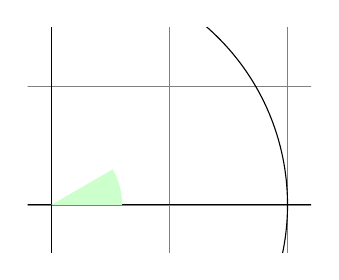
\begin{tikzpicture}[scale=3]
        \clip (-0.1,-0.2) rectangle (1.1,0.75);
        \draw[step=.5cm,gray,very thin] (-1.4,-1.4) grid (1.4,1.4);
        \draw (-1.5,0) -- (1.5,0);
        \draw (0,-1.5) -- (0,1.5);
        \draw (0,0) circle [radius=1cm];
        \fill[green!20!white] (0,0) -- (3mm,0mm)
            arc [start angle=0, end angle=30, radius=3mm] -- (0,0);
    \end{tikzpicture}
    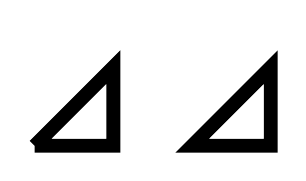
\begin{tikzpicture}[line width=5pt]
        \draw (0,0) -- (1,0) -- (1,1) -- (0,0);
        \draw (2,0) -- (3,0) -- (3,1) -- cycle;
        \useasboundingbox (0,1.5); % make bounding box higher
    \end{tikzpicture}
    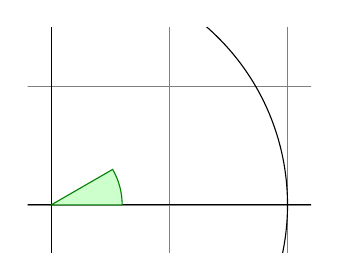
\begin{tikzpicture}[scale=3]
        \clip (-0.1,-0.2) rectangle (1.1,0.75);
        \draw[step=.5cm,gray,very thin] (-1.4,-1.4) grid (1.4,1.4);
        \draw (-1.5,0) -- (1.5,0);
        \draw (0,-1.5) -- (0,1.5);
        \draw (0,0) circle [radius=1cm];
        \filldraw[fill=green!20!white, draw=green!50!black] (0,0) -- (3mm,0mm)
            arc [start angle=0, end angle=30, radius=3mm] -- cycle;
    \end{tikzpicture}

    \item shading:
    
    \tikz \shade (0,0) rectangle (2,1) (3,0.5) circle (.5cm);
    
\begin{tikzpicture}[rounded corners,ultra thick]
        \shade[top color=yellow,bottom color=black] (0,0) rectangle +(2,1);
        \shade[left color=yellow,right color=black] (3,0) rectangle +(2,1);
        \shadedraw[inner color=yellow,outer color=black,draw=yellow] (6,0) rectangle +(2,1);
        \shade[ball color=green] (9,.5) circle (.5cm);
    \end{tikzpicture}

    \item 参考坐标:
    
    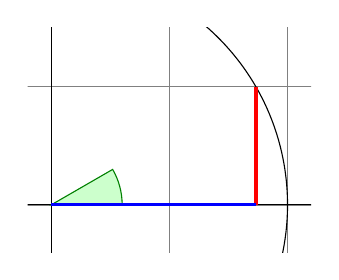
\begin{tikzpicture}[scale=3]
        \clip (-0.1,-0.2) rectangle (1.1,0.75);
        \draw[step=.5cm,gray,very thin] (-1.4,-1.4) grid (1.4,1.4);
        \draw (-1.5,0) -- (1.5,0);
        \draw (0,-1.5) -- (0,1.5);
        \draw (0,0) circle [radius=1cm];
        \filldraw[fill=green!20,draw=green!50!black] (0,0) -- (3mm,0mm)
        arc [start angle=0, end angle=30, radius=3mm] -- cycle;
        \draw[red,very thick] (30:1cm) -- +(0,-0.5);    % 参考坐标是 (30:1cm)
        \draw[blue,very thick] (30:1cm) ++(0,-0.5) -- (0,0);    % 参考坐标是 (30:1cm)+(0,-0.5)
    \end{tikzpicture}

    \item 通过参考坐标定义画 rectangle 的宏:
    
    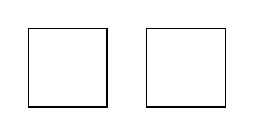
\begin{tikzpicture}
        \def\rectanglepath{-- ++(1cm,0cm) -- ++(0cm,1cm) -- ++(-1cm,0cm) -- cycle}
        \draw (0,0) \rectanglepath;
        \draw (1.5,0) \rectanglepath;
    \end{tikzpicture}
    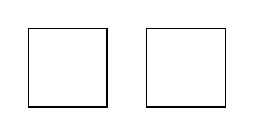
\begin{tikzpicture}
        \def\rectanglepath{-- +(1cm,0cm) -- +(1cm,1cm) -- +(0cm,1cm) -- cycle}
        \draw (0,0) \rectanglepath;
        \draw (1.5,0) \rectanglepath;
    \end{tikzpicture}
    \tikz \draw (0,0) rectangle +(1,1) (1.5,0) rectangle +(1,1);

    \item arrows:
    
    \item 正弦、余弦、正切:


\end{enumerate}


\end{document}
